\documentclass{standalone}
\usepackage{graphicx}	
\usepackage{amssymb, amsmath}
\usepackage{color}

\usepackage{tikz}
\usetikzlibrary{intersections, backgrounds, math}
\usepackage{pgfmath}

\definecolor{light}{RGB}{220, 188, 188}
\definecolor{mid}{RGB}{185, 124, 124}
\definecolor{dark}{RGB}{143, 39, 39}
\definecolor{highlight}{RGB}{180, 31, 180}
\definecolor{light_teal}{RGB}{107, 142, 142}
\definecolor{mid_teal}{RGB}{72, 117, 117}
\definecolor{dark_teal}{RGB}{29, 79, 79}
\definecolor{gray10}{gray}{0.1}
\definecolor{gray20}{gray}{0.2}
\definecolor{gray30}{gray}{0.3}
\definecolor{gray40}{gray}{0.4}
\definecolor{gray60}{gray}{0.6}
\definecolor{gray70}{gray}{0.7}
\definecolor{gray80}{gray}{0.8}
\definecolor{gray90}{gray}{0.9}
\definecolor{gray95}{gray}{0.95}


\begin{document}

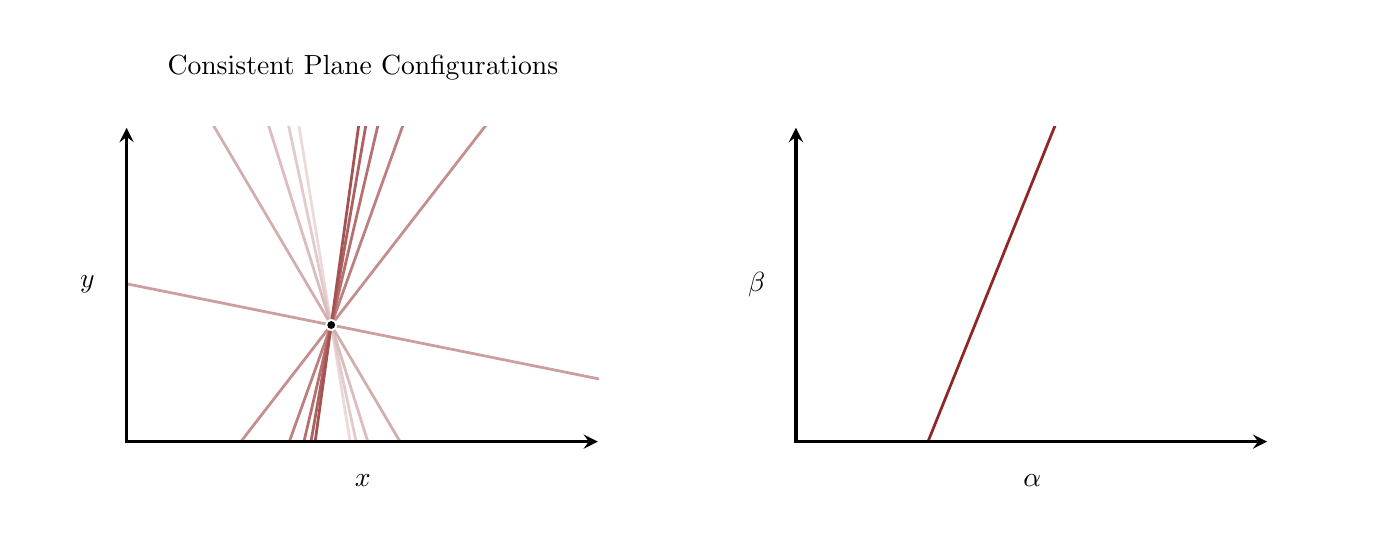
\begin{tikzpicture}[scale=1.0]

  \begin{scope}[shift={(0, 0)}]
    \draw[white] (-4.25, -3) rectangle (4.25, 3.25);  

    \node at (0, 2.75) { Consistent Plane Configurations };

    \begin{scope}
      \clip (-3, -2) rectangle (3, 2);
    
      \foreach \a [count=\n] in {-3, -2.4, ..., 3} {
        \pgfmathsetmacro{\b}{(-0.519 - \a) / -0.402};
        \pgfmathsetmacro{\prop}{10 + 7 * \n};
        \colorlet{custom}{dark!\prop!white};
        \draw[domain={-3:3}, smooth, samples=30, line width=1, variable=\x, color=custom] 
          plot ({\x},{\a + \b * \x});
      }
    
      \foreach \x/\y in {-0.402/-0.519} {
        \fill[white] (\x, \y) circle(0.075);
        \fill[black] (\x, \y) circle(0.05);
      }
    
    \end{scope}

    \draw [->, >=stealth, line width=1.25] (-3.00, -2.015) -- +(0, 4);
    \draw [->, >=stealth, line width=1.25] (-3.015, -2.00) -- +(6, 0);
    
    \node at (-3.5, 0) { $y$ };
    \node at (0, -2.5) { $x$ };
  \end{scope}
  
  \begin{scope}[shift={(8.5, 0)}]
    \draw[white] (-4.25, -3) rectangle (4.25, 3.25);  

    \begin{scope}
      \clip (-3, -2) rectangle (3, 2);
    
      \draw[domain={-3:3}, smooth, samples=30, line width=1, variable=\a, color=dark] 
          plot ({\a},{(-0.519 - \a) / -0.402});
    \end{scope}

    \draw [->, >=stealth, line width=1.25] (-3.00, -2.015) -- +(0, 4);
    \draw [->, >=stealth, line width=1.25] (-3.015, -2.00) -- +(6, 0);
    
    \node at (-3.5, 0) { $\beta$ };
    \node at (0, -2.5) { $\alpha$ };
  \end{scope}
  
\end{tikzpicture}

\end{document}  